Due to our limitation in computing resources, we can only present our approaches for the first 30 bins (meaning videos with age ranging from 1 day to 30 days). For each bin, we create 5 folds cross-validation with 80\% of our data for training, and the other 20\% for testing. The average results over 5-folds are reported.

We set the learning rate $\eta=1$, $\lambda=0.01$. The maximum of iteration is $maxIter=3$. We did try with other values of $maxIter$ up to 10, but they do not give significant gains and take more time to run.

\subsubsection{Classification Results}
	The accuracy and $F_1$-score of our logistic regression are presented in Table \ref{tbl:acc} and Table \ref{tbl:f1} correspondingly. For each metric, we present four approaches: original logistic regression (ORG), logistic regression with augmented features (AUG), logistic regression with weighed gradients (GRAD) and logistic regression with both extensions (BOTH). Each approach we compare with its corresponding ensemble version as described in section \ref{subsec:ext2}. 
	
Although all the approaches return barely above 50\%, there are some observations. First, the extension with augmented features have better performance than original approach. Meanwhile, the other extension with weighted gradient shows less effective in prediction.  That makes senses since we put more weights on the gradients, we have to employ a better control on the learning rate. Otherwise the parameters would oscillate over the optimal points. It also explains the 'BOTH' method performs the worst in accuracy and $F_1$-scores.
	
Secondly, most of the ensemble methods have better performance (both in accuracy and $F_1$-scores) than single predictions. That supports our hypothesis that by partitioning the videos into bins, we worsen the sparseness in each bin's data. Hence by using an weighted combination of all classifiers, we can pass information between the bins to achieve better performance. Recall that the ensemble methods work only if all the individual predictors have good performance in their own data. Since 'BOTH' and 'GRAD' have lower accuracy in prediction, ensemble methods do not work in their cases. That explains the exceptional observations in $F_1$-scores when the single predictors of both perform better.
		
			\begin{table}[h]
			\caption{Average of Accuracy over 5 folds of 30 bins.}
			\label{tbl:acc}
				\begin{center}
					\begin{tabular}{| l | c | c |}						
					\hline
					Approach & Single Predictor & Ensemble \\ \hline
					BOTH & 0.513 & \textbf{0.526} \\ \hline
					GRAD & 0.514 & \textbf{0.527} \\ \hline
					AUG & 0.516 & \textbf{0.534} \\ \hline
					ORG & 0.514 & \textbf{0.532} \\ \hline		
					\end{tabular}
				\end{center}	
			\end{table}

	\begin{table}[h]
	\caption{Average of $F_1$-score over 5 folds of 30 bins.}
	\label{tbl:f1}
		\begin{center}		
			\begin{tabular}{| l | c | c |}
			\hline
				Approach & Single Predictor & Ensemble \\ \hline
				BOTH & \textbf{0.468} & 0.463 \\ \hline
				GRAD & \textbf{0.451} & 0.443 \\ \hline
				AUG & 0.473 & \textbf{0.503} \\ \hline
				ORG & 0.455 & \textbf{0.468} \\ \hline
			\end{tabular}
		\end{center}
	\end{table}
	
\subsubsection{Regression Results}
	The linear regression can be evaluated in more than one way.
	
	The first way to measure our results is to look at its predictions directly.  Our mean squared error indicated that our prediction was was typically 0.93 orders of magnitude away from the true result, but it is hard to say whether we should be impressed.
	
	The second form of evaluation is to compare the results for each pair of videos and then use the \textbf{0-1 loss function}, so that results can be compared to the logistic regression results.  Not surprisingly, logistic regression performed better (having been trained explicitly for this task).  What is surprising, however, is that our accuracy is not significantly greater than 50\%, which indicates that our linear regression holds no measurable value for the ranking problem.
	
	A likely cause is that this problem may not be linear in nature -- in fact, it would admittedly be surprising if it were.  We tested our accuracy on the training data as well as on the testing data, and found that it performed just as poorly, indicating that the weak results on our testing data did not stem from over fitting.
	
	In order to investigate further, we plotted our output against the true number of views (for a random subset of our data):

	\begin{figure}[!h]
		\begin{center}
			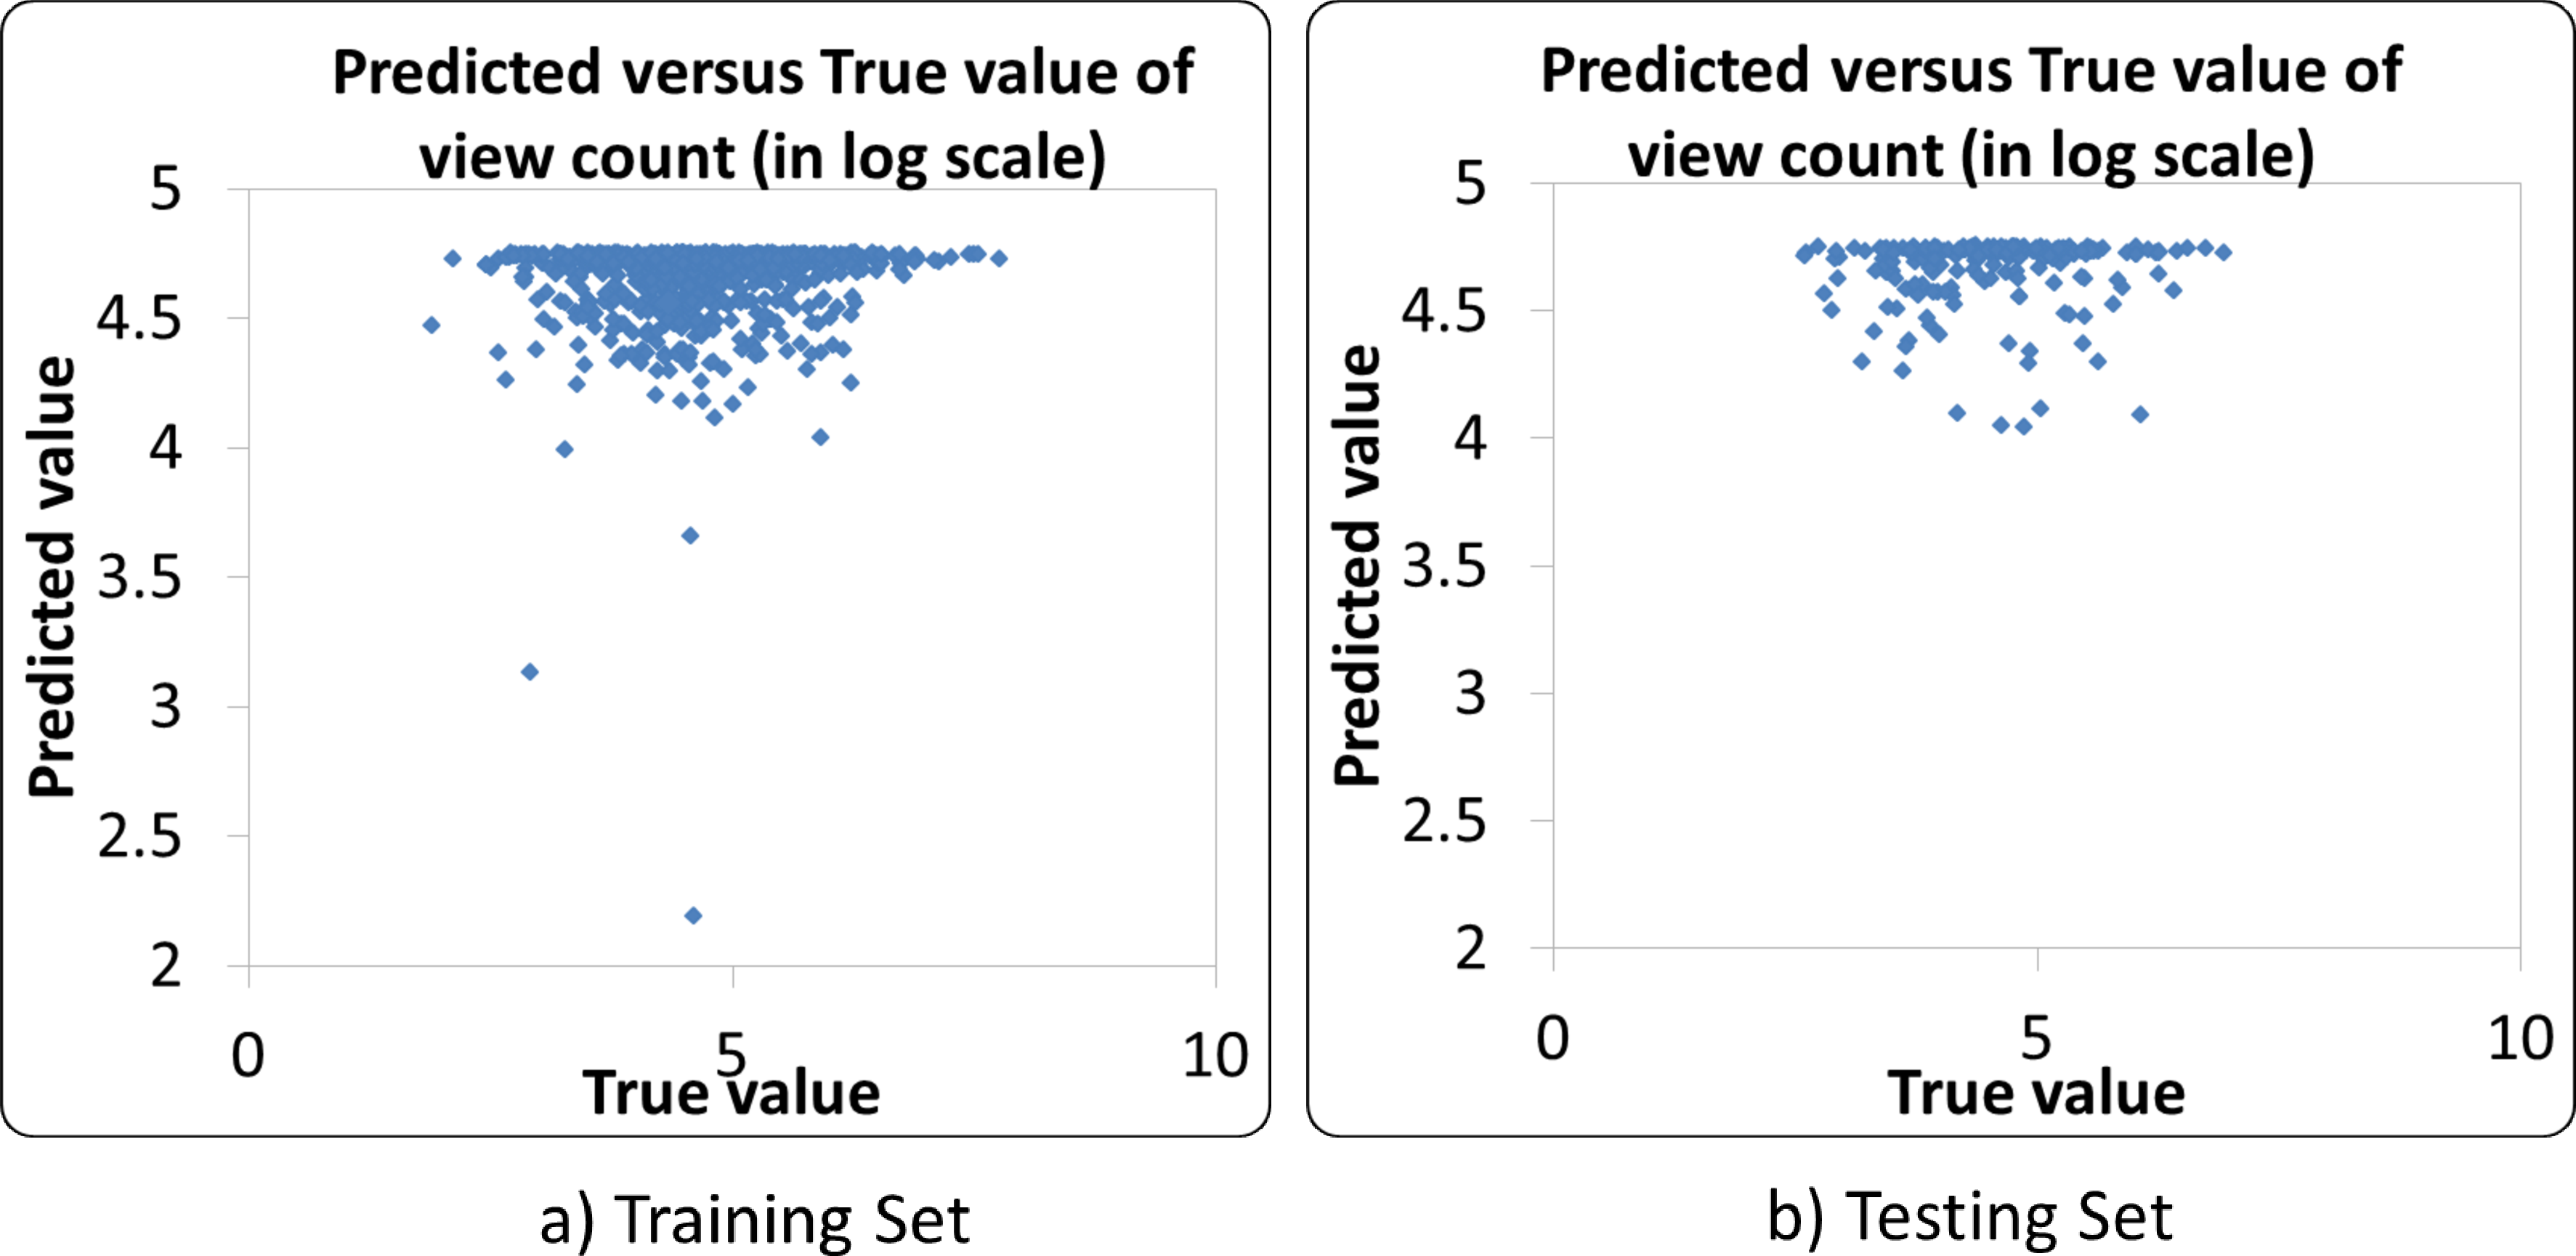
\includegraphics[width=.75\textwidth,clip]{regression.pdf}
		\end{center}
		\caption{True value vs prediction (in log-scale).}
		\label{fig:trainingTrueVsPredicted}
	\end{figure}
		
	We observe a strong tendency towards the same output value (roughly 50,000 views), which corresponds to the average number of views -- this would be the typical outcome when linear regression is inadequate.
